\documentclass[]{tufte-book}

% ams
\usepackage{amssymb,amsmath}

\usepackage{ifxetex,ifluatex}
\usepackage{fixltx2e} % provides \textsubscript
\ifnum 0\ifxetex 1\fi\ifluatex 1\fi=0 % if pdftex
  \usepackage[T1]{fontenc}
  \usepackage[utf8]{inputenc}
\else % if luatex or xelatex
  \makeatletter
  \@ifpackageloaded{fontspec}{}{\usepackage{fontspec}}
  \makeatother
  \defaultfontfeatures{Ligatures=TeX,Scale=MatchLowercase}
  \makeatletter
  \@ifpackageloaded{soul}{
     \renewcommand\allcapsspacing[1]{{\addfontfeature{LetterSpace=15}#1}}
     \renewcommand\smallcapsspacing[1]{{\addfontfeature{LetterSpace=10}#1}}
   }{}
  \makeatother

\fi

% graphix
\usepackage{graphicx}
\setkeys{Gin}{width=\linewidth,totalheight=\textheight,keepaspectratio}

% booktabs
\usepackage{booktabs}

% url
\usepackage{url}

% hyperref
\usepackage{hyperref}

% units.
\usepackage{units}


\setcounter{secnumdepth}{2}

% citations
\usepackage{natbib}
\bibliographystyle{plainnat}

% pandoc syntax highlighting

% longtable
\usepackage{longtable,booktabs}

% multiplecol
\usepackage{multicol}

% strikeout
\usepackage[normalem]{ulem}

% morefloats
\usepackage{morefloats}


% tightlist macro required by pandoc >= 1.14
\providecommand{\tightlist}{%
  \setlength{\itemsep}{0pt}\setlength{\parskip}{0pt}}

% title / author / date
\title{Book Template}
\author{Caltech Library}
\date{2020-10-07}

\usepackage{booktabs}
\usepackage{amsthm}
\makeatletter
\def\thm@space@setup{%
  \thm@preskip=8pt plus 2pt minus 4pt
  \thm@postskip=\thm@preskip
}
\makeatother

\begin{document}

\maketitle



{
\setcounter{tocdepth}{1}
\tableofcontents
}

\chapter{Introduction}\label{introduction}

Welcome to a demo of using bookdown to create an electronic textbook.

\section{Markdown syntax}\label{markdown-syntax}

Markdown is a simple text-based way of formatting documents. There are
many flavors of markdown, we'll start with standard markdown and then
add some specific rmarkdown information. Let's look at some other
basics:

\begin{itemize}
\tightlist
\item
  You can put text into \emph{italics} and \textbf{bold} using * or **
\item
  To create headings, put one or more \# symbols at the beginning of a
  line, followed by a space. One \# is for a level one header, \#\# for
  a level two header, etc.
\item
  To make bullet lists (such as this one), just start lines with a -;
  you can get additional levels by starting a line a couple of spaces or
  a tab in. Numbered lists work the same way using 1. 2. 3.
\end{itemize}

\begin{verbatim}
    - Topic 1
    - Topic 2  
    - Topic 3
      - Topic 3a
\end{verbatim}

\begin{itemize}
\item
  To cite code (including markdown syntax as above) use ` on both sides
  for short bits and ``` in a separate line above and below larger
  codeblocks.
\item
  Quote text using \textgreater{} at the beginning of the line (maybe
  you remember this from old e-mail programs?)
\end{itemize}

\texttt{\textgreater{}\ This\ is\ a\ Quote}

\begin{itemize}
\tightlist
\item
  A link is set putting the text that you want to highlight in square
  brackets followed by the link in round brackets. Don't forget to
  include \url{http://} or \url{https://} at the beginning of the link
\end{itemize}

\texttt{{[}This\ is\ a\ link{]}(http://www.example.com)}

You can find more markdown formatting options
\href{https://bookdown.org/yihui/rmarkdown/markdown-syntax.html}{here}.
Note that markdown comes in different dialects, referred to as
``flavors''. The basic elements above are part of a consensus referred
to as \href{http://commonmark.org/}{Common Markdown}, though some of the
more advanced options we'll discuss later are specific to Rmarkdown.

\hypertarget{methods}{\chapter{Methods}\label{methods}}

\section{Citations and Citation
Styles}\label{citations-and-citation-styles}

\section{Bookdown Specific Features}\label{bookdown-specific-features}

You can label chapter and section titles using \texttt{\{\#label\}}
after them, e.g., we can reference Chapter \ref{introduction}. If you do
not manually label them, there will be automatic labels anyway, e.g.,
Chapter \ref{methods}.

\section{Including Code and Images}\label{including-code-and-images}

\subsection*{Schematic: Bactofilin}\label{Bactofilin}
\addcontentsline{toc}{subsection}{Schematic: Bactofilin}

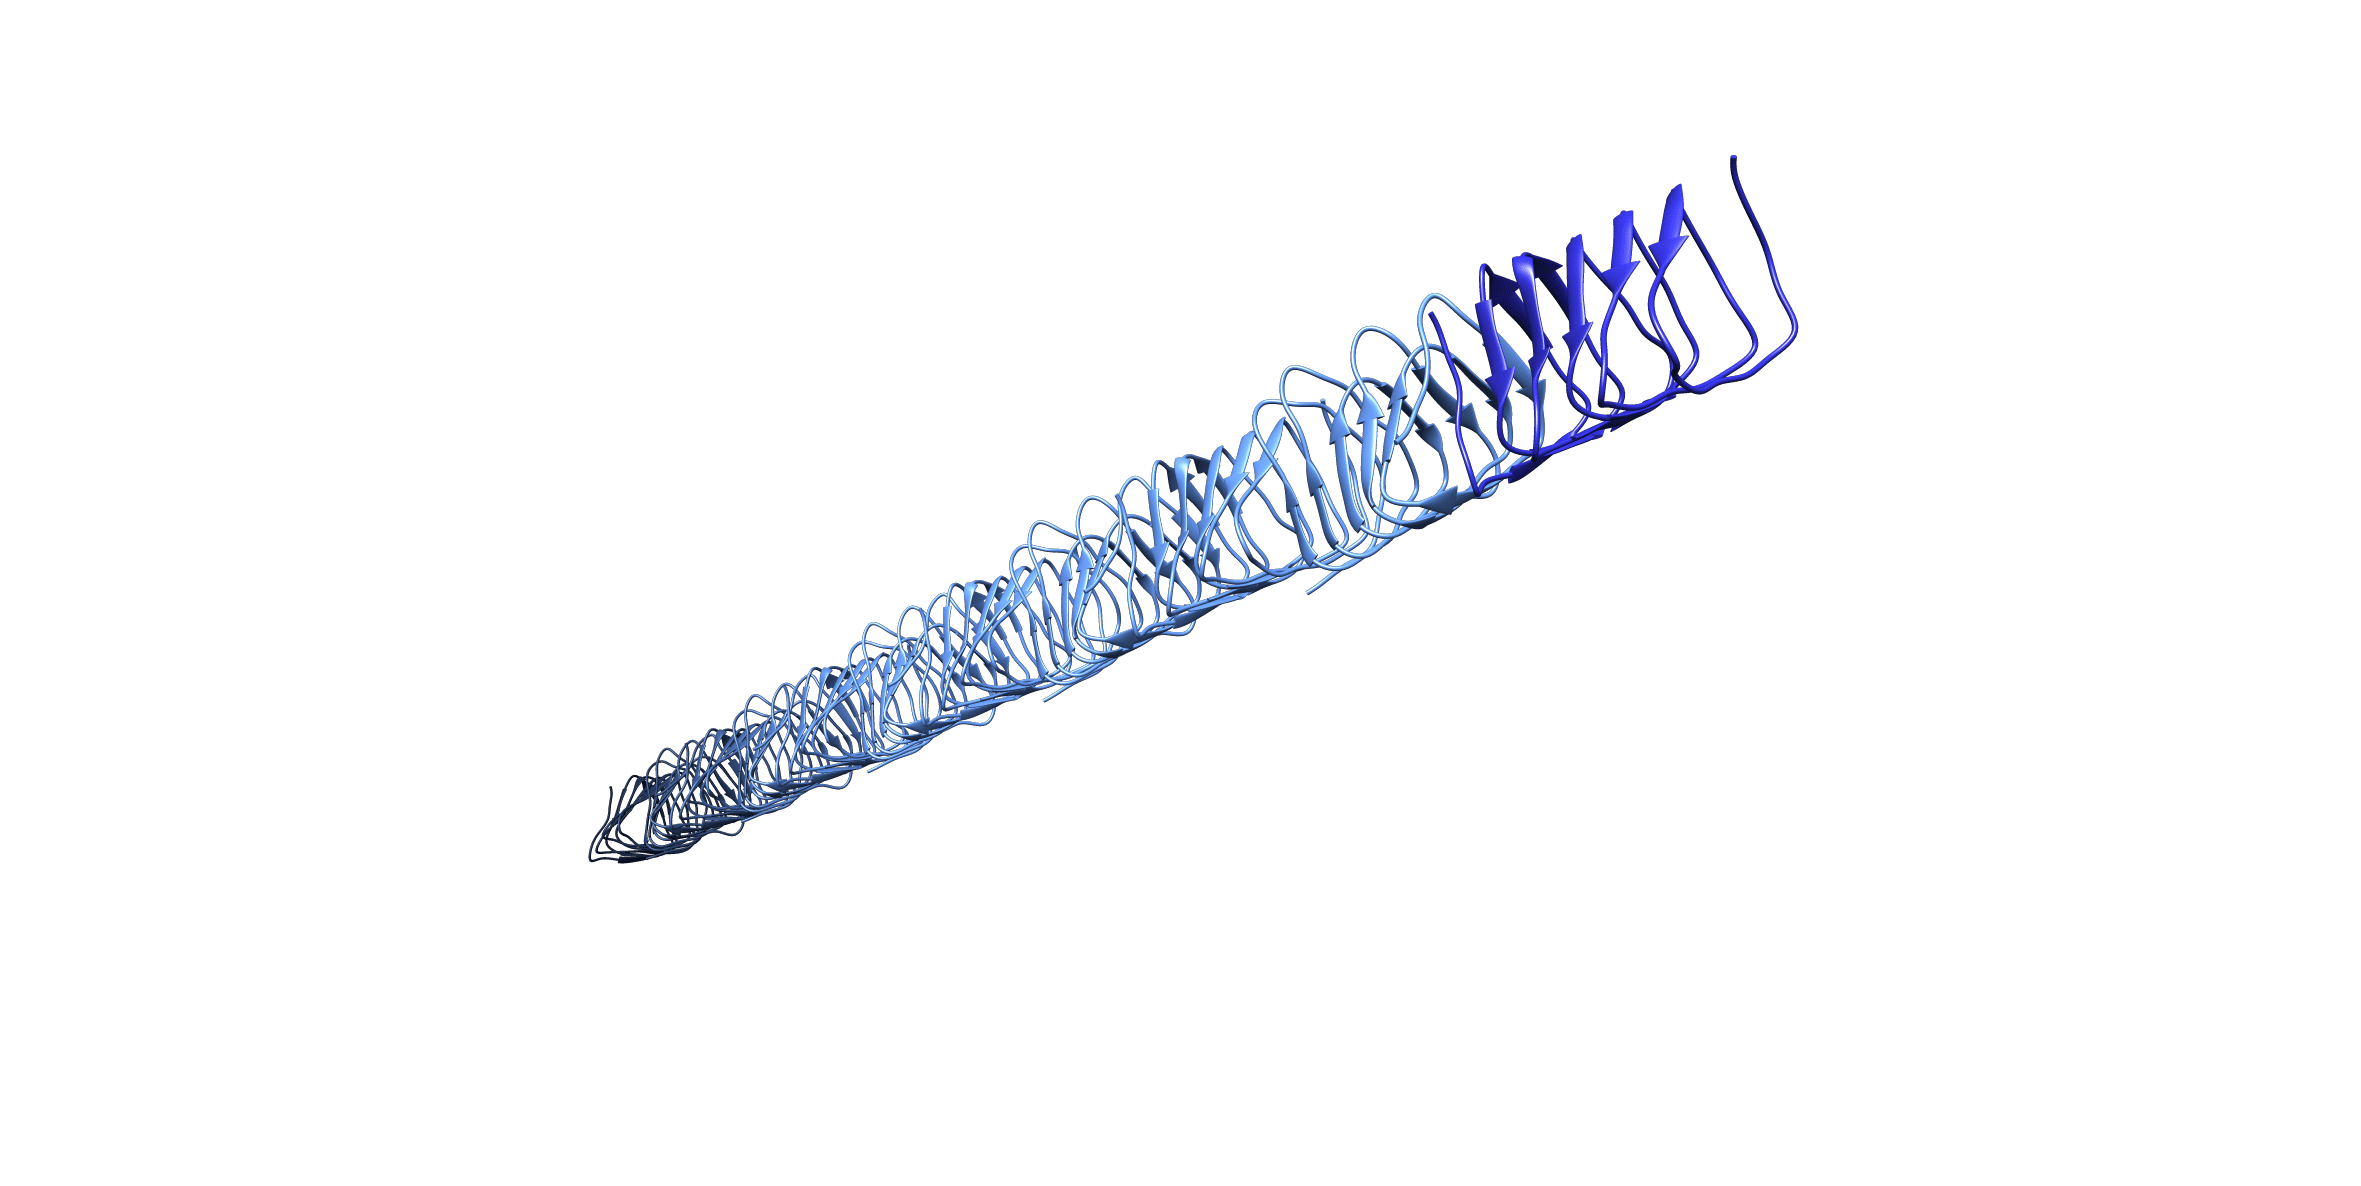
\includegraphics{img/3_6_1}

\href{http://rcsb.org/structure/6RIB}{\emph{PDB: 6RIB}} Bactofilins are
found in many species of bacteria and archaea, suggesting that they
perform diverse (and currently unknown) functions. They polymerize into
very stable filaments with a triangular beta-helical structure, like
this one from \emph{Thermus thermophilus} \citep{deng2019}. Bactofilin
filaments lack two hallmarks of actin- and tubulin-based cytoskeletal
elements: polarity and dynamic assembly/disassembly. In this way, they
are similar to intermediate filaments in eukaryotic cytoskeletons.

\section{LaTeX}\label{latex}

\section{Caltech Custom Features}\label{caltech-custom-features}

If you have a video on CaltechDATA, we can add embed it using just the
DOI. This example also shows how you can define a caption using a ()
label outside of am element, let Bookdown format it, and them embed it





\begin{figure}
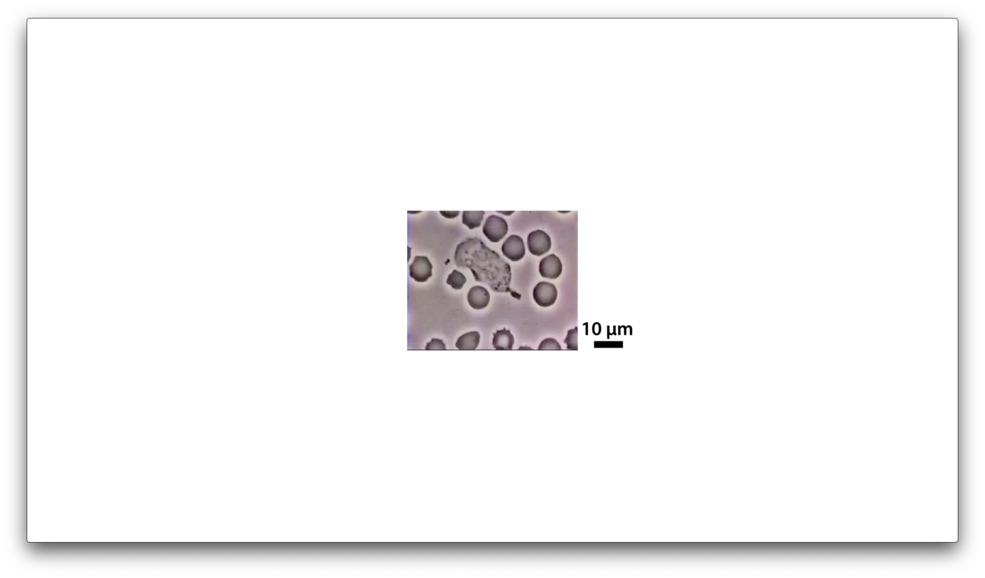
\includegraphics{movie_stills/1_1} \caption[\protect\hyperlink{methods}{Staphylococcus aureus} Collected
by: David Rogers Movie DOI:
\href{https://doi.org/10.22002/D1.1463}{10.22002/D1.1463}]{\protect\hyperlink{methods}{Staphylococcus aureus} Collected
by: David Rogers Movie DOI:
\href{https://doi.org/10.22002/D1.1463}{10.22002/D1.1463}}\label{fig:1-1}
\end{figure}

We also provide a method for embeddig video files locally, if you want
the book to work offline.

\begin{figure}
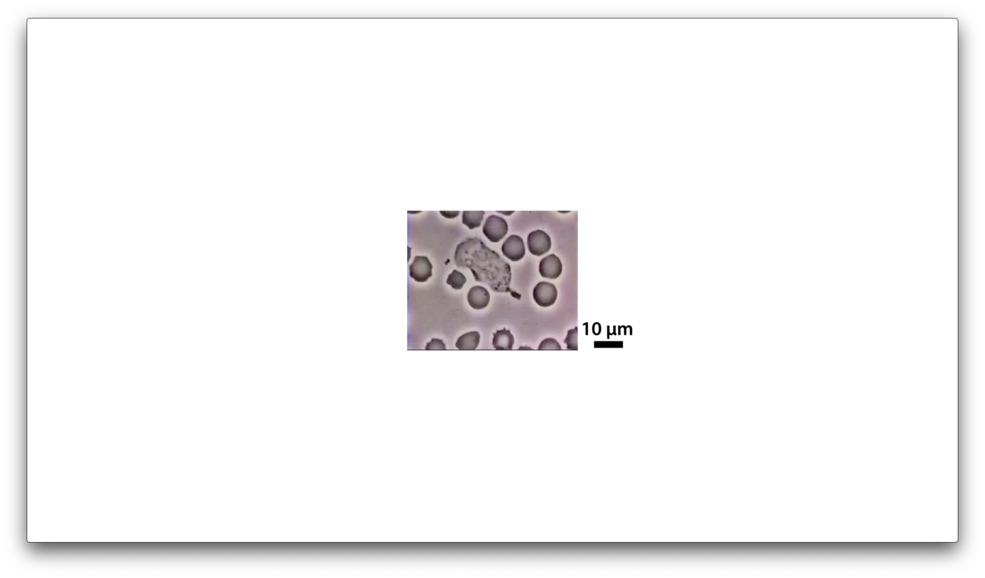
\includegraphics{movie_stills/1_1} \caption[\protect\hyperlink{methods}{Staphylococcus aureus} Collected
by: David Rogers Movie DOI:
\href{https://doi.org/10.22002/D1.1463}{10.22002/D1.1463}]{\protect\hyperlink{methods}{Staphylococcus aureus} Collected
by: David Rogers Movie DOI:
\href{https://doi.org/10.22002/D1.1463}{10.22002/D1.1463}}\label{fig:1-1-embed}
\end{figure}

\subsection*{Further Reading}\label{further-reading}
\addcontentsline{toc}{subsection}{Further Reading}

Errington (2013). \emph{L-form bacteria, cell walls and the origins of
life} \citep{errington2013}.

Ptacin and Shapiro (2013). \emph{Chromosome architecture is a key
element of bacterial cellular organization} \citep{ptacin2013}.

Sleytr and Beveridge (1999). \emph{Bacterial S-layers}
\citep{sleytr1999}.

Strahl and Errington (2017). \emph{Bacterial membranes: Structure,
domains, and function} \citep{strahl2017}.

\bibliography{AtlasBibTeX.bib}



\end{document}
